
\chapter{Science Writing Heuristic eller at skrive for at lære}
 \label{app:A}
 
 Hvis du spørger dine klassekammerater eller din underviser efter en definition på begrebet \emph{undersøgelse}, vil du formentlige få ligeså mange forskellige unikke definitioner som antallet af personer du har spurgt. Dette skyldes at \emph{undersøgelse} kan have mange forskellige meninger uafhængigt af personen der spørges. I denne laboratorie manual, har vi valgt følgende forståelse af begrebet \emph{undersøgelse} som midlerne til at gennemføre videnskab. For at hjælpe dig til at tænke hele vejen igennem den videnskabelige process har vi struktureret denne manual med overskrifter som er draget ud fra pricippet science writing heuristic (SWH).
 
SWH er en velbeskrevet metode til at styre undersøgelsesbaserede oplevelser, og den er designet til at opfordre til konstruktion af konceptuel viden i faget. Metoden er også baseret på sammenhængen mellem spørgsmål, evidens og påstande. Den oprindelige udgave af science writing heuristic inkluderede følgende processer som du som elev skal igennem.
 
 \begin{enumerate}
 	\item Første spørgmål til undersøgelsen\vspace{-15pt}
 	\item Test\vspace{-15pt}
 	\item Observationer\vspace{-15pt}
 	\item Påstande\vspace{-15pt}
 	\item Evidens\vspace{-15pt}
 	\item Læsning\vspace{-15pt}
 	\item Refleksion\vspace{-15pt}
 	\item Skrive fase
\end{enumerate}

Ovenstående otte kategorier er blevet tilpasset arbejdet med undersøgelser, således at de nu er følgende overskrifter. Under hver af overskrifterne finder du en kort instruks, som forholder sig til den undersøgelse som relaterer sig til overskrifter. Overskrifterne kobler også til de faglige mål i fysik faget.

\section{Stil spørgsmål}
\label{sec:SS}
Enhver videnskabelig undersøgelse begynder normalvis med en undren der kan formuleres som et spørgsmål. Dette spørgsmål skal så besvares gennem eksperimenter hvor man indsamler data. Fra tid til anden er dette spørgsmål givet på forhånd, mends det andre gange vil være dig der skal stille spørgsmålet sammen med din laboratorie gruppe.

\section{Forberedelse af undersøgelse}
 \label{sec:FaU}
 Før du kan påbegynde dit praktiske arbejde, er det vigtigt at der er en klar plan for hvordan du vil indsamle dine data, som skal danne grundlaget for din evidens senere. Dette inkluderer også at indetificere hvilke data der skal indsamles og hvilke skridt der skal følges i laboratoriet. I nogle tilfælde vil, en fuldstændig eller delvis procedure være indkluderet i vejledningen til undersøgelsen. I de fleste tilfælde skal du dog udlede dele af eller hele proceduren sammen med din laboratoriegruppe. Uanset om proceduren er givet eller du skal lave den, skal du studere den nøje forud for det praktiske arbejde. Du er også nødt til at fremstille et system til at nedfælde observationer og målinger fra undersøgelsen - fx en tabel eller et skema enten på papir eller i excel.
 
 \section{Lav forudsigelser}
 \label{sec:LF}
 I langt de fleste undersøgelser, bør du prøve at forudsige hvad du forventer der sker når du indsamler evidens. Disse forudsigelser skal være baseret på dine egne erfaringer og vil på ingen måde blive vurderet for deres korrekthed, men du kan med fordel reflektere over dem efter at have gennemført det praktiske arbejde - passer din forståelse med det eksperimentet viser?
 
 \section{Indsamling af empiri}
 \label{sec:IaE}
 Hjørnestenen i enhver undersøgelse er indsamlingen af empiri som danner grundlaget for den evidens som senere skal underbygge dine påstande. Når du indsamler empiri skal du være opmærksom på at få alle tal noteret korrekt i det skema/den tabel du har lavet til formålet. Endvidere skal du sørge for at notere alt hvad du observerer. Dette kan indeholde retninger, skridt foretaget i undersøgelsen, eller en guide til indsamling af empiri og øvrige observationer.
 
 \section{Analyse af empiri}
 \label{sec:AaE}
 Den indsamlede empiri vil i de fleste tilfælde kræve at du foretager yderligere behandling af data før du kan svarer på dit oprindelige spørgsmål fra afsnit \vref{sec:SS}. Inden du går i krig med din empiri bør du kigge på dine data og se om der er noget som springer i øjnene fx punkter som afviger klart fra de øvrige eller generelle tendenser som fremstår klart fra den indsamlede empiri. Herefter bør du foretage de nødvendige beregninger eller en grafisk analyse af den indsamlede empiri. Her vil det være fint at vise et regne eksempel med et eller to datapunkter. Resultatet af din analyse er den evidens som skal underbygge de påstande du har fremhævet baseret på den indsamlede empiri.
 
 \section{Fortolkning af evidens}
\label{sec:FaE}
Når du har analyseret din empiri, og nu har noget evidens, bør du altid spørge dig selv, ``Hvad betyder denne evidens?'' For at kunne besvarer dette spørgmål, er du nødt til at foreslå forklaringer/påstande på de videnskabelige fænomener. Spørgsmål i dette afsnit er designet for at hjælpe dig med at tænke over de konsekvenser som evidensen medfører og at rette eller korrigere denne til et meningsfuldt formål med undersøgelsen.

\section{Fremstilling af påstande}
\label{sec:FaP}
Når du er i mål med en analyse og en fortolkning af din empiri, og du har fremsat et svar på dit indledende spørgsmål. Bør du omformulere dette til en videnskabelig påstand. En sådan påstand skal altid kunne underbygges med evidensen fra undersøgelsen. Når du har fremstillet påstande bør du kigge i litteraturen for at underbygge dem med andres viden.

\section{Reflektion over undersøgelsen}
\label{sec:RoU}
Den afsluttende opgave i de fleste undersøgelser er at reflektere over hvad der blev gjort, overvej hvordan din forståelse har udviklet sog, og anvend din nye viden på andre lignende situationer.

\section{Noter}
Det er mit håb at denne manual vil kunne hjælpe dig i forarbejdet til dit skriftlige arbejde med undersøgelser, og at den ligeledes vil hjælpe dig til at blive en bedre videnskabsmand. Denne instruktion er sammensat af viden fra \citep{Hand2004, Greenbowe2005, Krogh2016}


\chapter{Nyttevirkning af elkedel og kaffemaskine}
\label{app:B}

\section{Formål}
Formålet med øvelsen er at bestemme den nyttevirkning, hvormed nogle almindelige elektriske apparater omsætter elektrisk energi. I dette tilfælde undersøges en elkedel og en kaffemaskine.

\section{Teori}
Når man benytter et elektrisk apparat, vil en del af den elektriske energi, der omsættes, gå til spilde. Opvarmer man f.eks. vand i en kedel, bruges en del af den tilførte elektriske energi til opvarmning af kedlen og omgivelserne.
Ved nyttevirkningen eller effektiviteten (betegnes med det græske bogstav $\eta$ (eta)) af et apparat forstår man forholdet mellem den udnyttede energi og den tilførte energi angivet i procent:
\begin{equation*}
	\eta = \frac{\Delta E_{\mathrm{nyt}}}{\Delta E_\mathrm{til}}\cdot 100 \%
\end{equation*}
$\Delta E_\mathrm{til}$ er i denne øvelse den elektriske energi, som et apparat omsætter. Derfor udregner man $\Delta E_\mathrm{til}$ ved hjælp af formlen:
\begin{equation*}
\Delta E_\mathrm{til} = P\cdot \Delta t
 \end{equation*}
hvor $P$ er apparatets effektforbrug og $\Delta t$ er den tid, hvor apparatet er tændt.
$\Delta E_{\mathrm{nyt}}$ er den energi, som udnyttes til opvarmning af vandet. Når vi har en mængde vand med massen $m$, kan denne energi beregnes ved hjælp af formlen:
\begin{equation*}
\Delta E_{\mathrm{nyt}} = m\cdot c\cdot \Delta T = m\cdot c\cdot (T_{2} – T_{1})
\end{equation*}
hvor $c$ er den specifikke varmekapacitet (varmefylde) for vand. $c$ har værdien \mbox{4180 $\joule\per(\kilo\gram\cdot\celsius)$}.
$T_1$ og $T_2$ er vandets begyndelses- og sluttemperatur.

Bemærk, at vi i denne øvelse bruger symbolet $t$ for tid og $T$ for temperatur.

\section{Apparatur}
Elkedel, kaffemaskine, stopur, måleglas, termometer, effektmåler, vægt.

\section{Opstilling}
Tegn selv opstillingen eller tag et billede af den.

\section{Udførelse}
\begin{itemize}
	\item[1)] {\bfseries Elkeden:}
	Der afmåles ca. 1,0 kg vand i elkedlen. Effektmåleren sættes i stikkontakten, og elkedlen kobles til effektmåleren. Vandets begyndelsestemperatur $T_{1}$ aflæses. Elkedlen og stopuret tændes samtidig. På effektmåleren aflæses den effekt, hvormed der omsættes elektrisk energi. Når vandet koger, antager i at sluttemperaturen $T_2$ er 100 \celsius, hvilket i noterer i jeres skema. Den forløbne tid $\Delta t$ noteres.
	\item[2)] {\bfseries Kaffemaskienen:}
	Målingerne forløber som ved elkedlen. Vandets sluttemperatur er temperaturen af det vand, der er løbet ned i kaffemaskinen. Tidtagningen slutter, når alt vandet er løbet igennem og i aflæser sluttemperaturen $T_2$. På effektmåleren aflæses den effekt, hvormed der omsættes elektrisk energi.
\end{itemize}

\section{Måleresultater}
\begin{table}
\centering
\caption[Data registreringsskema]{pris/kWh = \hspace{5cm} $c$ =}
\label{tbl:data.forsøg1}
\begin{tabular}{ @{ } p{3cm}  p{3cm}  p{3cm} @{ } }
	\toprule[2pt]
			&	Elkedel	&	Kaffemaskine	\\
	\midrule[1.2pt]
	$m (\kilo\gram)$					&			&				\\
	$T_{1} (\celsius)$					&			&				\\
	$T_{2} (\celsius)$					&			&				\\
	$\Delta T (\celsius)$					&			&				\\
	$\Delta E_{\mathrm{nyt}} (\joule)$		&			&				\\
	$P (\watt)$						&			&				\\
	$\Delta t (\second)$					&			&				\\
	$\Delta E_{\mathrm{til}} (\joule)$		&			&				\\
	$\eta (\%)$						&			&				\\
	$\Delta E_{\mathrm{til}} (\kilo\watt\hour)$	&			&				\\
	Pris (kroner)						&			&				\\
	\bottomrule[2pt]
\end{tabular}
\end{table}

\section{Databehandling}
\begin{enumerate}
	\item De tomme rubrikker i skemaet udfyldes og medtages i rapporten. Og der vises eksempler på udregninger for elkedlen i de efterfølgende spørgsmål.
	\item Udregning af temperaturtilvæksten $\Delta T$.
	\item Udregning af den udnyttede energi  $\Delta E_{\mathrm{nyt}}$
	\item Udregning af den tilførte energi $\Delta E_{\mathrm{til}}$
	\item Udregning af nyttevirkningen $\eta$
	\item Udregning af den tilførte energi $\Delta E_{\mathrm{til}}$ i \kilo\watt\hour
	\item Udregning af prisen for at opvarme vandet.
\end{enumerate}
Du må naturligvis gerne bruge kaffemaskinen i stedet for elkedlen til at vise eks. på udregninger. Du skal så blot angive det.

\section{Diskussion}
Diskuter resultaterne. Man kan f.eks. komme ind på følgende spørgsmål:
\begin{itemize}
	\item Hvilket af de to apparater udnytter den elektriske energi bedst?
	\item Hvilke fordele og ulemper kan man nævne ved hvert af de to apparater, når de bruges til at lave \'en liter kaffe?
	\item Hvad er prisen for den elektriske energi, der omsættes, når man laver én liter kaffe henholdsvis på kaffemaskinen og ved hjælp af elkedlen?
\end{itemize}

 \section{konklusion}

\chapter{Undersøgelse af diffraktion}
\label{app:C}
Hvis man betragter den problemstilling som eleverne i gruppen med elev 4 havde under forsøget med fænomenet diffraktion af laserlys. Så kan det diskuteres om eleverne har de fornødne færdigheder til at kunne foretage en fyldestgørende analyse af problemet i forhold til at frembringe evidens og rygdæknig for en påstand. 
Udgangspunktet er følgende eksperimentelle opstilling se figur \firef{ops.app}
\begin{figure}[h!]
	\centering
	\begin{tikzpicture}
		%\draw[very thin, blue!25, step=1mm, anchor=south east] (0,0) grid (12,6);
		%\draw[blue!50, step=5mm, anchor=south east] (0,0) grid (12,6);
		%\draw[thick, blue!75, step=10mm, anchor=south east] (0,0) grid (12,6);
		
		\draw[thick, black] (7,2.5) arc (0:12:1.9cm);
		\draw[thick, black] (7.5,2.5) arc (0:23:2.4cm);
		
		\filldraw[fill=white,draw=black, thick] (0,2.25) -- (2,2.25) -- (2,2.75) -- (0,2.75) -- cycle;
		\draw[very thick, red] (2,2.5) -- (12,2.5) node[black,right] {$n = 0$};
		\draw[very thick, fill=red,draw=red] (12,2.5) circle (1mm);
		
		\draw[very thick, red] (5.1,2.5) -- (12,4) node[black,right] {$n = 1$};
		\draw[very thick, fill=red,draw=red] (12,4) circle (1mm);
		
		\draw[very thick, red] (5.1,2.5) -- (12,5.5) node[black,right] {$n = 2$};
		\draw[very thick, fill=red,draw=red] (12,5.5) circle (1mm);
		
		\draw[very thick, draw=black,fill=black] (4.9,1) rectangle (5.1,4) node[above] {Gitter};
		
		\node at (6.75,2.75) {$\theta_1$};
		\node at (7.75,2.75) {$\theta_2$};
		\node at (1,2.5) {Laser};
		\draw[very thick, black, <-] (5.1,1.5) -- (8,1.5);
		\draw[very thick, black, ->] (9,1.5) -- (12,1.5);
		\node at (8.5,1.5) {$L$};
		\draw[very thick, black, <-] (12,2.6) -- (12,3);
		\draw[very thick, black, ->] (12,3.5) -- (12,3.9);
		\node at (12,3.24) {$S_1$};
	\end {tikzpicture}
	\caption[Eksperimentel opstilling]{Forsøgsopstillingen til eksperimenterne som eleverne har udført dem.}
	\label{fig:ops.app}
\end{figure}

Her får eleverne brug for at anvende en tangensrelation til at bestemme afbøjningsvinklen $\theta_n$ til den $n$'te orden. 
\begin{equation}
	\theta_n = \tan^{-1}\left(\frac{S_n}{L}\right)
\end{equation}
her er $S_n$ afstanden mellem 0'te og $n$'te orden i interferensmønstret mens $L$ er afstanden mellem gitteret og målepunktet som vist på figur \firef{ops.app}. Denne værdi for vinklen indsættes på vinklens plads i gitterligningen.
\begin{equation}
	d\cdot\sin\theta_n = n\cdot \lambda
\end{equation}
hvor $d$ er gitterkonstanten, $n$ er ordensnummeret dvs et positivt heltal og $\lambda$ er laserens bølgelængde. Nu indsættes udtrykket for afbøjningsvinklen $\theta_n$ i ligningen herover of der isoleres for afstanden mellem ordenerne herved finder man følgende udtryk:
\begin{equation}
	S_n = \tan\left(\sin^{-1}\left(\frac{n\cdot\lambda}{d}\right)\right)\cdot L
\end{equation}
Modelleres dette udtryk i et matematik program med passende valg af $n$, $d$, $\lambda$ og $L$ kan man få figur \firef{eviden.app}. 
\begin{figure}[h!]
	\centering
	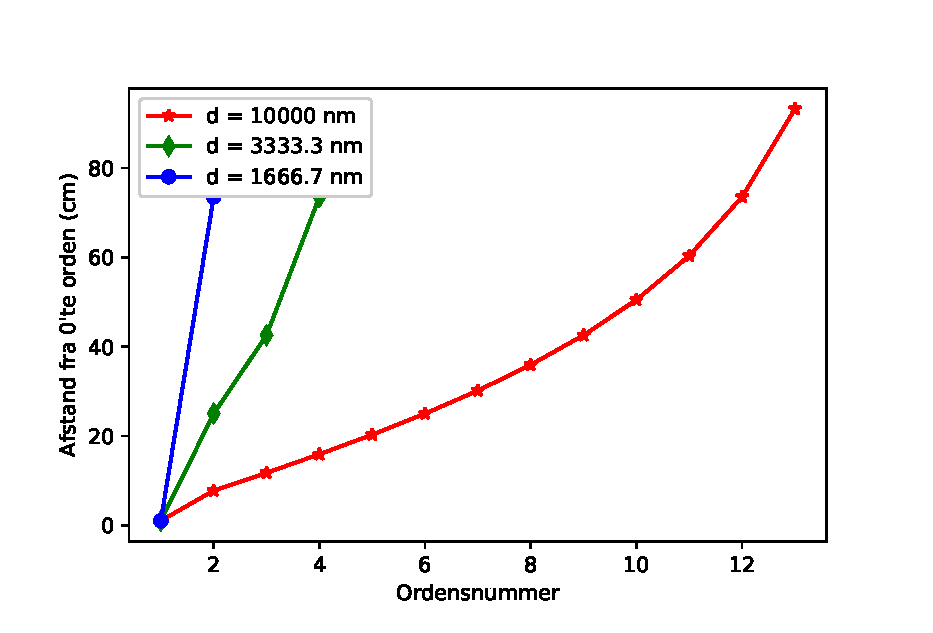
\includegraphics[width=\textwidth]{Figs/test}
	\caption[Eksempel på teoretisk modellering]{Her ses en teoretisk modelleret udgave af figur \firef{evidens.jacob} som gruppen med elev 4 frambragte eksperiementelt på baggrund af de data de havde til rådighed. På figuren er gitteret med 600 linjer\per\milli\meter~plottet med en blå (dot-dash) line, gitteret med 300 linjer\per\milli\meter~er plottet med en grønd stiplet linje og gitteret med 100 linjer\per\milli\meter~er plottet med en fuldtoptrukken rød linje.}
	\label{fig:eviden.app}
\end{figure}

Her illusrerer den blå linje et gitter med 600 linjer pr mm, den grønne et gitter med 300 linjer pr mm mens den røde viser et gitter med 100 linjer pr mm. Heraf ses det at gruppen med elev 4 faktisk har ramt den overordnede trent ret godt, omend deres afstande er temmelig meget for små, i forhold til den teoretiske model som er vist her. 